\documentclass[wide,a4paper,titlepage,12pt] {article}
\usepackage{polski}
\usepackage[utf8]{inputenc}
\usepackage{listings}
\usepackage{placeins}
\usepackage{graphicx}



\title{Sterowniki mikroprocesorowe w aplikacjach sieciowych}
\author{Tymon Tobolski (181037)\\ Jacek Wieczorek (181043)}

% Title page layout (fold)
\makeatletter
\renewcommand{\maketitle}{
\begin{titlepage}
  \begin{center}
    \vspace*{3cm}
    \LARGE \@title \par
    \vspace{2cm}
    \textit{\small Autor:}\par
    \normalsize \@author\par \normalsize
    \vspace{3cm}
    \textit{\small Prowadzący:}\par
    Dr inż. Jerzy Greblicki \par
    \vspace{2cm}
    Wydział Elektroniki\\ III rok\\ Cz TP 12.15 - 15.00\par

  \end{center}
\end{titlepage}
}
\makeatother
  \lstset{
    language=c++,
    basicstyle=\ttfamily\scriptsize,
    numbers=left,
    numberstyle=\scriptsize,
    stepnumber=10,
    numbersep=9pt,
    showspaces=false,
    showstringspaces=false,
    showtabs=false,
    breaklines=true,
  }

\begin{document}
\maketitle
  \section{Cel laboratorium}
  \paragraph{}
  Celem laboratorium było zapoznanie się z zasadą działania tranzystorów bipolarnych (pnp i npn) oraz MOSFET.

  \section{Układ 1}
  \paragraph{}
  Moc na tranzystorze \texttt{npn} w czasie otwarcia : \texttt{12 mW}

  \begin{figure}[h!]
  \begin{center}
  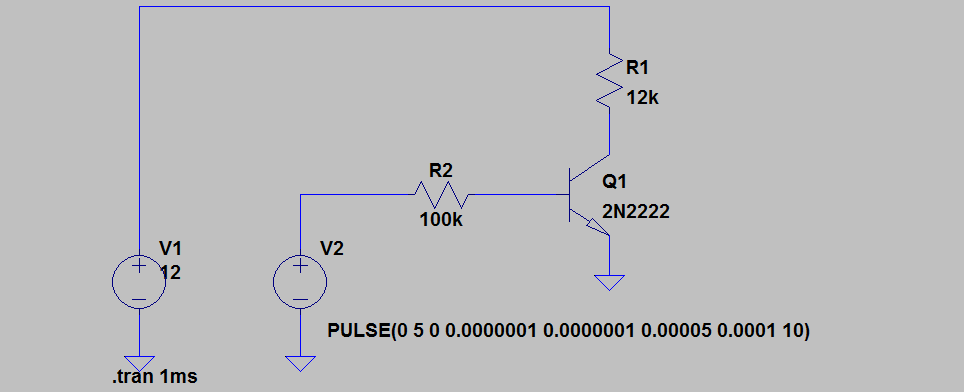
\includegraphics[scale=.5]{ukl1-npn.PNG}
  \caption{Układ npn}
  \label{fig:main}
  \end{center}
  \end{figure}  

\newpage

  \section{Układ 2}
  \paragraph{}
  Moc na tranzystorze \texttt{Q1} : \texttt{0.192 mW}
  Moc na tranzystorze \texttt{Q2} : \texttt{1.21 mW}

  \begin{figure}[h!]
  \begin{center}
  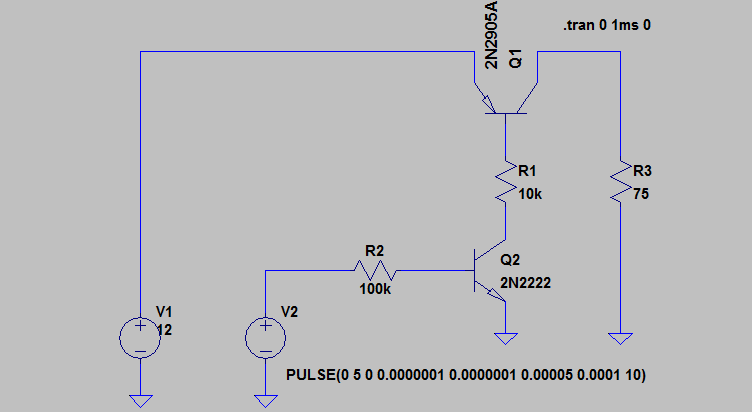
\includegraphics[scale=.5]{ukl2-pnp.PNG}
  \caption{Układ pnp}
  \label{fig:main}
  \end{center}
  \end{figure}

\newpage

  \section{Układ 3}
  \paragraph{}
  Moc na tranzystorze \texttt{M1} : \texttt{1.44 mW}
  Moc na tranzystorze \texttt{M2} : \texttt{1.08 mW}
    \begin{figure}[h!]
  \begin{center}
  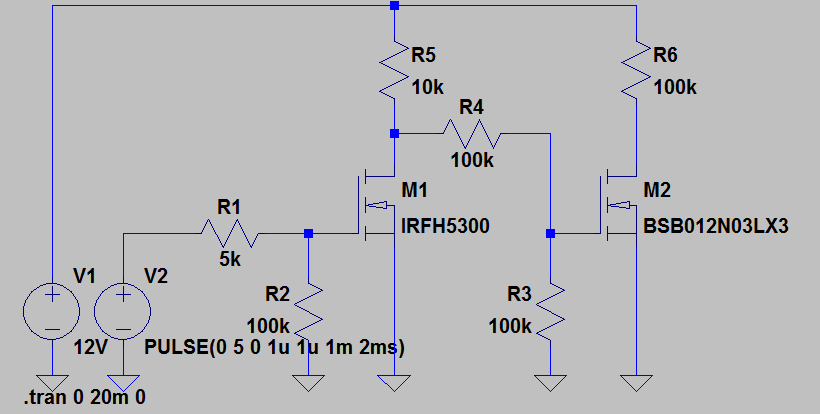
\includegraphics[scale=.5]{ukl3.PNG}
  \caption{Układ trzeci}
  \label{fig:main}
  \end{center}
  \end{figure}

\newpage

  \section{Układ 4}
  \paragraph{}
  Nie udało nam się uzyskać układu mającego na wyjściu 1mA, daltego zamieszczamy obliczenia dla poniższego układu.
  Moc na tranzystorze \texttt{M1} : \texttt{41.3 mW}
  Moc na tranzystorze \texttt{M2} : \texttt{0.78 mW}

  \begin{figure}[h!]
  \begin{center}
  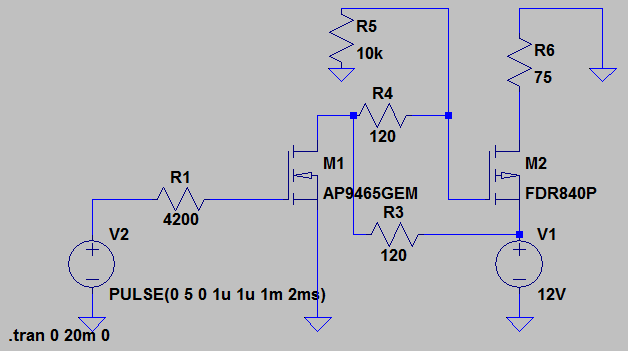
\includegraphics[scale=.5]{p4.png}
  \caption{Układ czwarty}
  \label{fig:main}
  \end{center}
  \end{figure}


\end{document}
